\chapter{探索性数据分析}

本章将会向你展示如何使用数据变形和绘图探索数据。统计学家称之为探索性数据分析或 \texttt{EDA}。EDA 实际上是个循环的工作,在 EDA 中你经常需要重复下面的三个环节:

\begin{enumerate}
\item 提出有关数据的问题;
\item 通过数据处理和可视化搜寻答案;
\item 使用你搜寻到的答案提出新的问题。
\end{enumerate}

EDA 并没有一个正规的流程。最重要的是,EDA 是一种好的工作习惯,它可以帮助你了解数据,发现一些简单想法的答案。在 EDA 的初始阶段,你可以随意探索一些你觉得有意思的问题,其中有一些想法你会得到正确的答案,而有些则会失败。

EDA 是任何数据分析的重要组成部分。要进行数据清理,你需要部署 EDA 的所有工具:可视化、转形和建模。

\section{问题}

在 EDA 期间的目标是了解数据。最简单的方法是使用问题作为指导探索的工具。当你提出问题的时候,问题会将你的注意力集中在数据机的特定部分,并帮助你的确定要生成的图形、模型。

EDA 从根本上来说是一个创造性的过程。在分析开始的时候很难提出问题,因为你不知道数据集中包含哪些信息。另一方面,你提出的每个新问题都会让你了解数据中包含的新信息,并且增加你发掘信息的机会。你可以快速深入查看数据中最有趣的部分,并开发一组发人深省的问题------如果你根据所发现的内容跟进每个问题并提出新问题。

有两种类型的问题对于数据探索是非常有用的:
\begin{enumerate}
  \item 我的变量中出现了什么类型的变化?
  \item 我的变量之间发生了什么类型的协变?
\end{enumerate}

本章的其余部分将讨论这两个问题。我将解释变异和协变是什么,我将向你展示几种回答每个问题的方法。

\section{变化}
\subsection{可视化分布}

如何可视化变量的分布取决于变量是分类变量还是连续变量。如果变量只能采用一小组值中的一个,则该变量是分类的。在 R 中,分类变量通常保存为因子或字符变量。要检查分类变量的分布,可以使用条形图,绘图结果见图 \ref{fig:histogramcut}。

\begin{lstlisting}
use diamonds, clear
histogram cut, freq barwidth(0.8)
\end{lstlisting}

\begin{figure}[htbp]
  \centering
  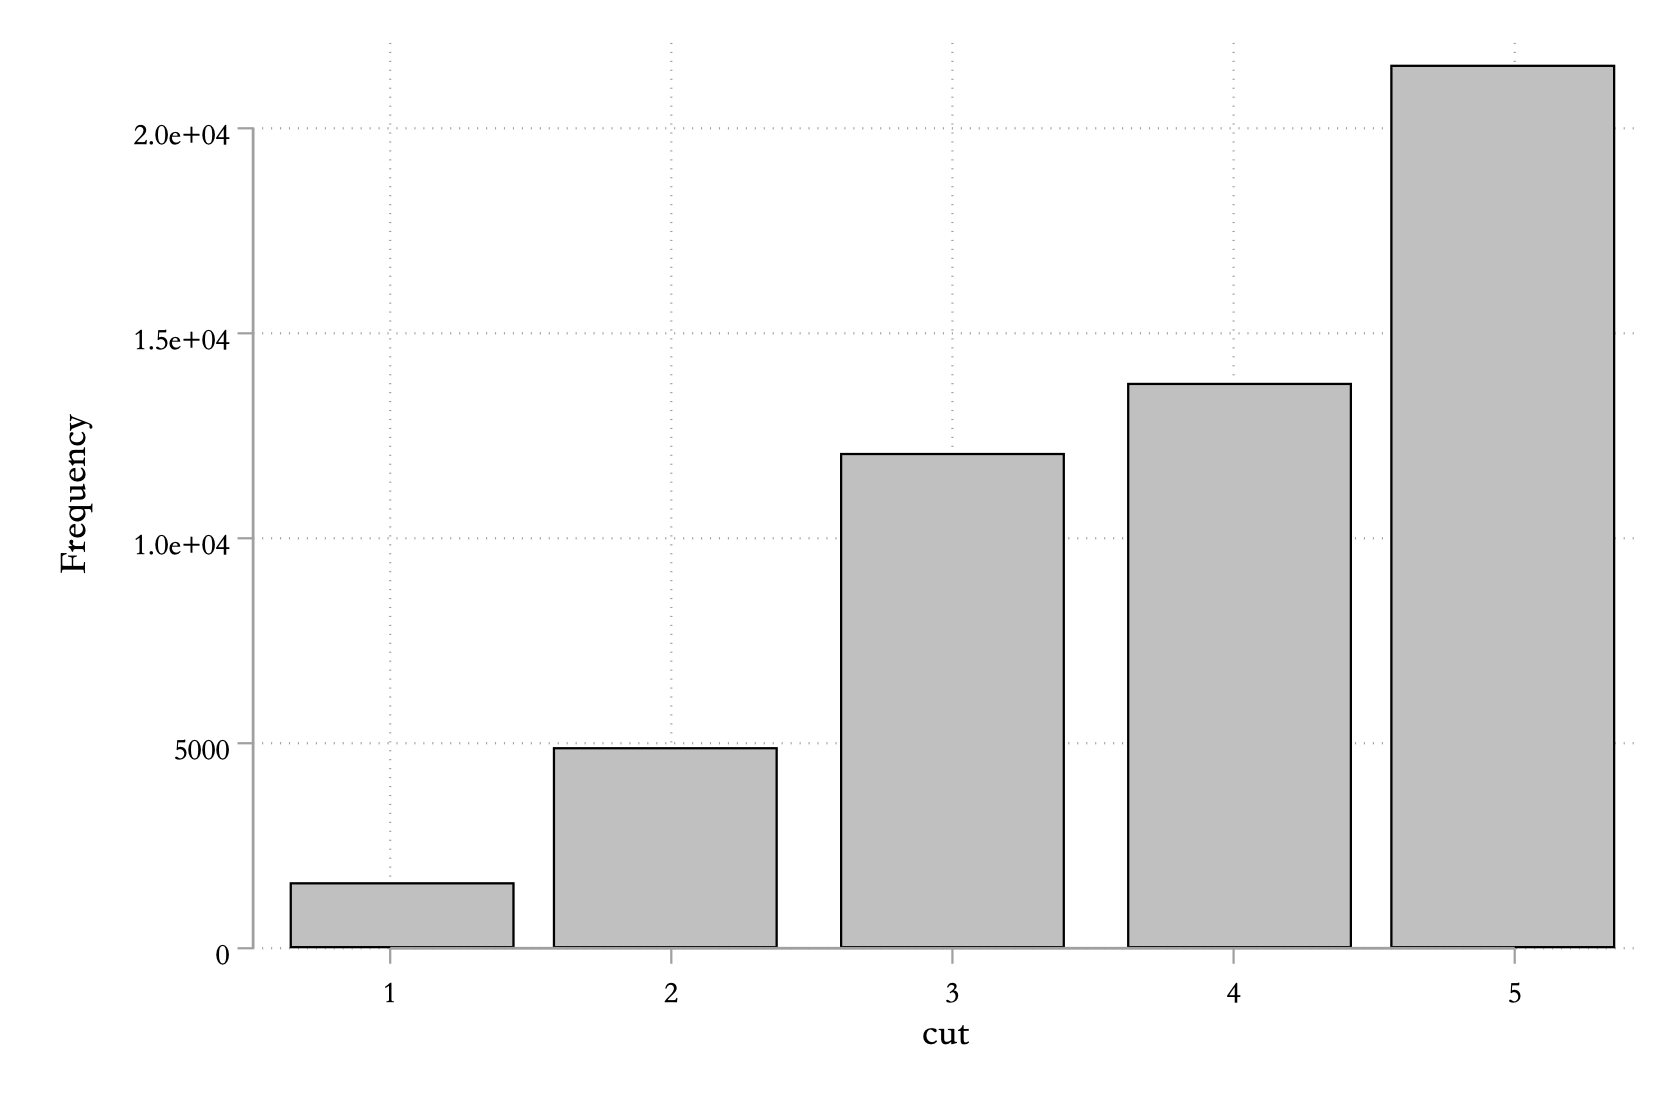
\includegraphics[width=\textwidth]{assets/histogramcut.png}
  \caption{cut 变量的分布}
  \label{fig:histogramcut}
\end{figure}

由于这里我设定了 \texttt{freq} 选项,所以纵轴显示的是频数。另外你也可以手动计算 cut 变量每个因子的观测值的数目然后绘图:

\begin{lstlisting}
use diamonds, clear
contract cut
tw bar _freq cut
\end{lstlisting}

\begin{figure}[htbp]
  \centering
  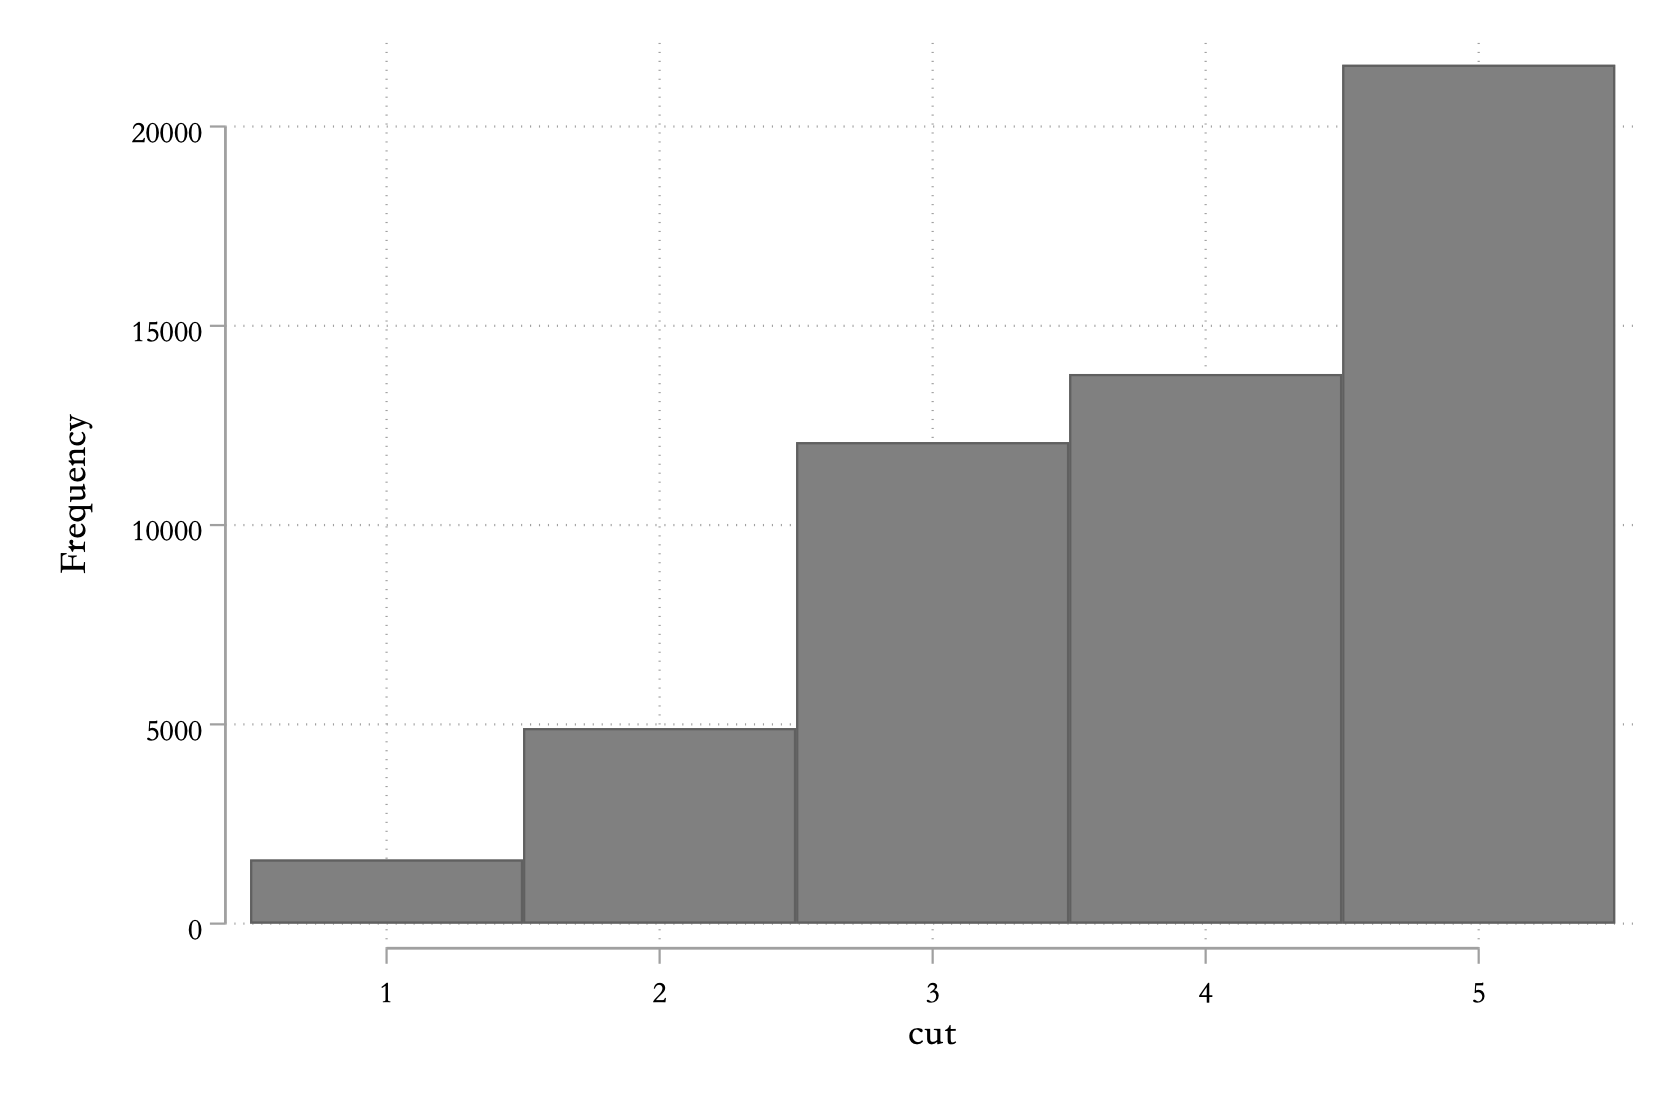
\includegraphics[width=\textwidth]{assets/histogramcut2.png}
  \caption{cut 变量的分布}
  \label{fig:histogramcut2}
\end{figure}

如果变量可以在连续集上进行取值,那么该变量就是连续的。数字和日期变量就是连续变量的两个例子。要检查连续变量的分布,请使用直方图:

\begin{lstlisting}
use diamonds, clear
hist carat, freq
\end{lstlisting}

\begin{figure}[htbp]
  \centering
  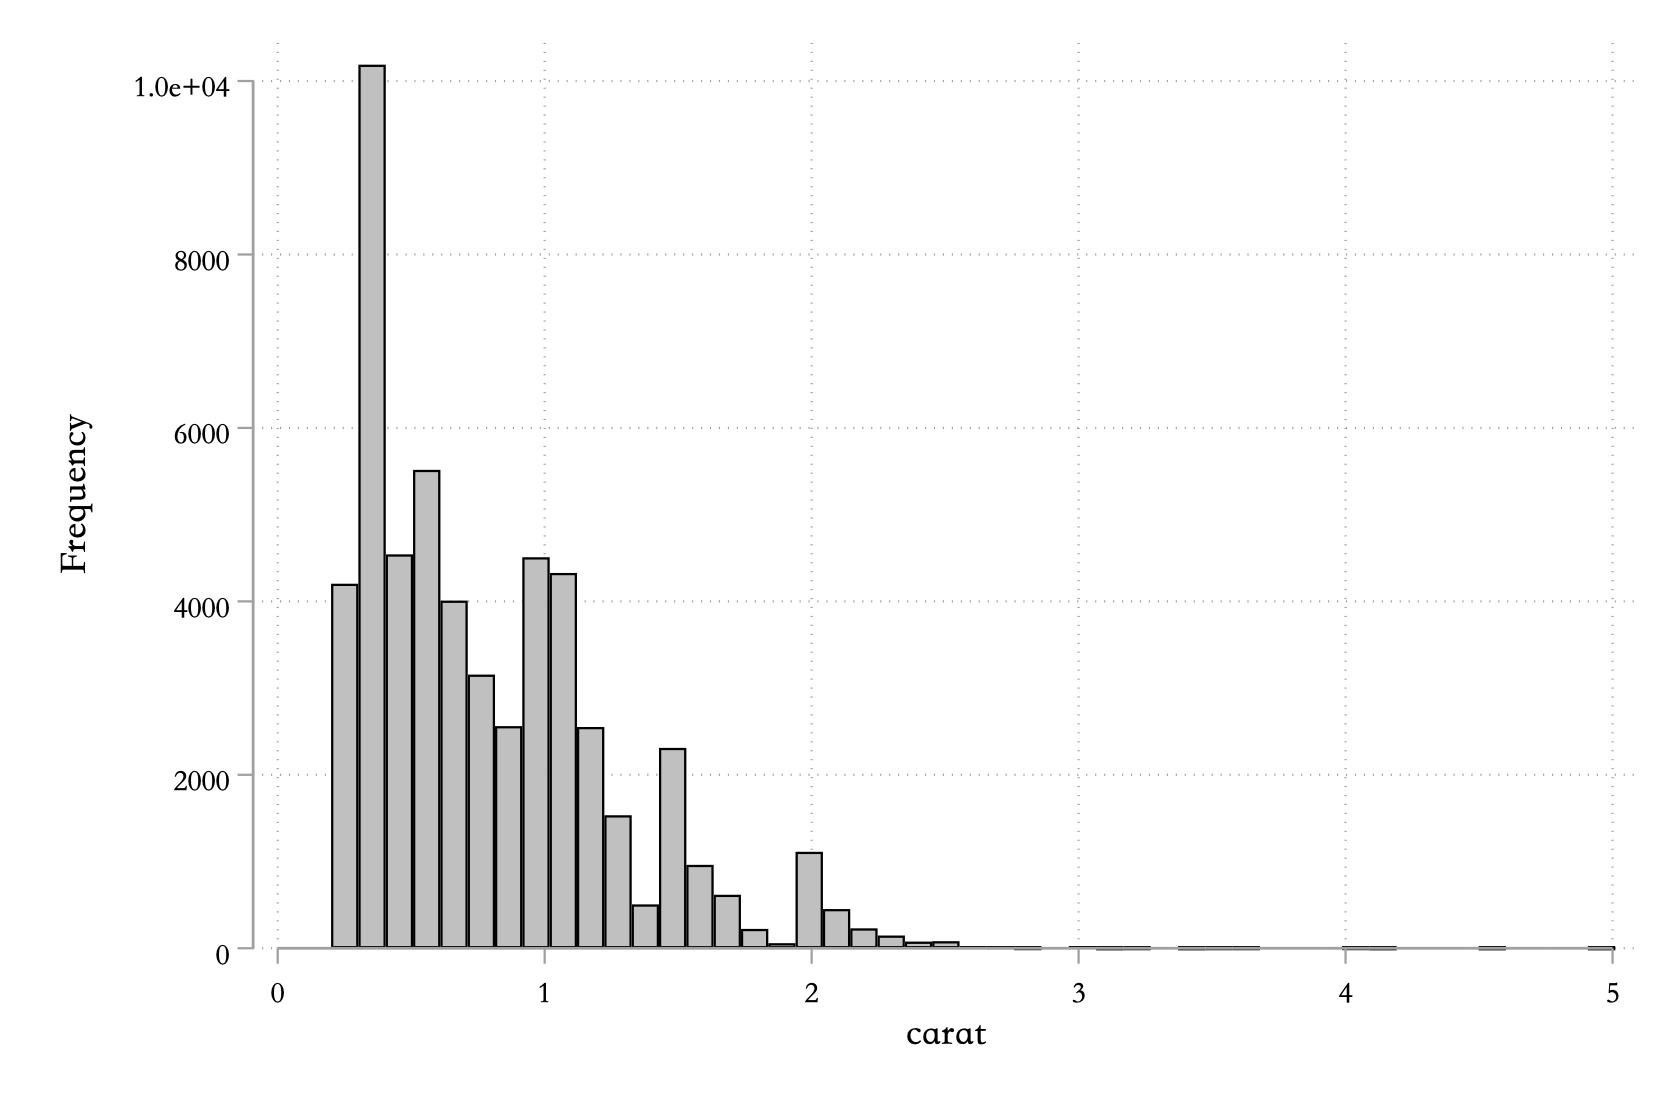
\includegraphics[width=\textwidth]{assets/histcarat.png}
  \caption{carat 变量的分布}\label{fig:histcarat}
\end{figure}

你可以使用 \texttt{width(0.5)} 指定每组组宽为 0.5 :

\begin{lstlisting}
hist carat, freq width(0.5)
\end{lstlisting}

\begin{figure}[htbp]
  \centering
  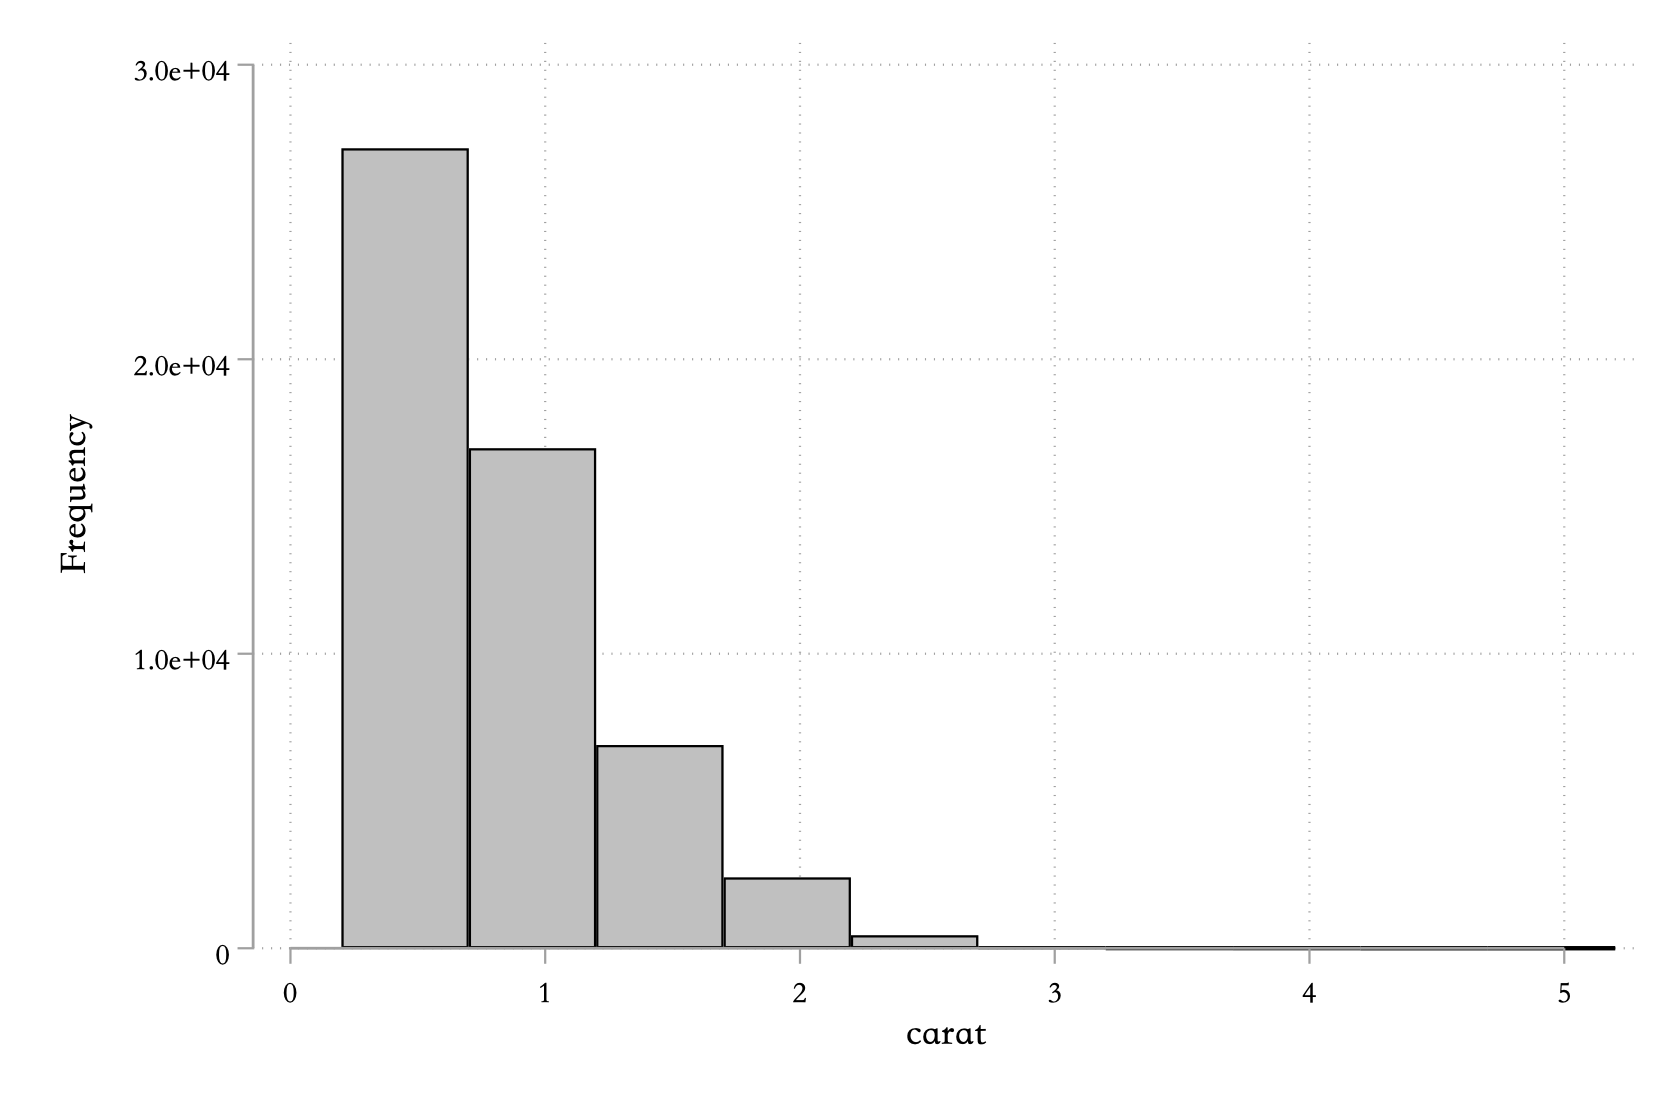
\includegraphics[width=\textwidth]{assets/histcarat2.png}
  \caption{carat 变量的分布}
  \label{fig:histcarat2}
\end{figure}

直方图将 x 轴分成等间距的箱,然后使用条的高度显示每个箱子中的观测数。在上图中,最高的条形显示近 3000 个观测值的 carat 变量值介于 0.25 和 0.75 之间,这是条形图的左右边界。

\texttt{width()} 选项可以用来设置组宽,该选项是以 x 变量为单位进行测量的。在使用直方图的时候,你应该始终探索各种带宽,因为不同的宽度可以揭示不同的模式,例如图\ref{fig:histsmallercarat}是我们放大 carat \textless{} 3 的钻石并选择较小的宽度绘制的直方图:

\begin{lstlisting}
use diamonds, clear
keep if carat < 3
hist carat, width(0.1)
\end{lstlisting}

\begin{figure}[htbp]
  \centering
  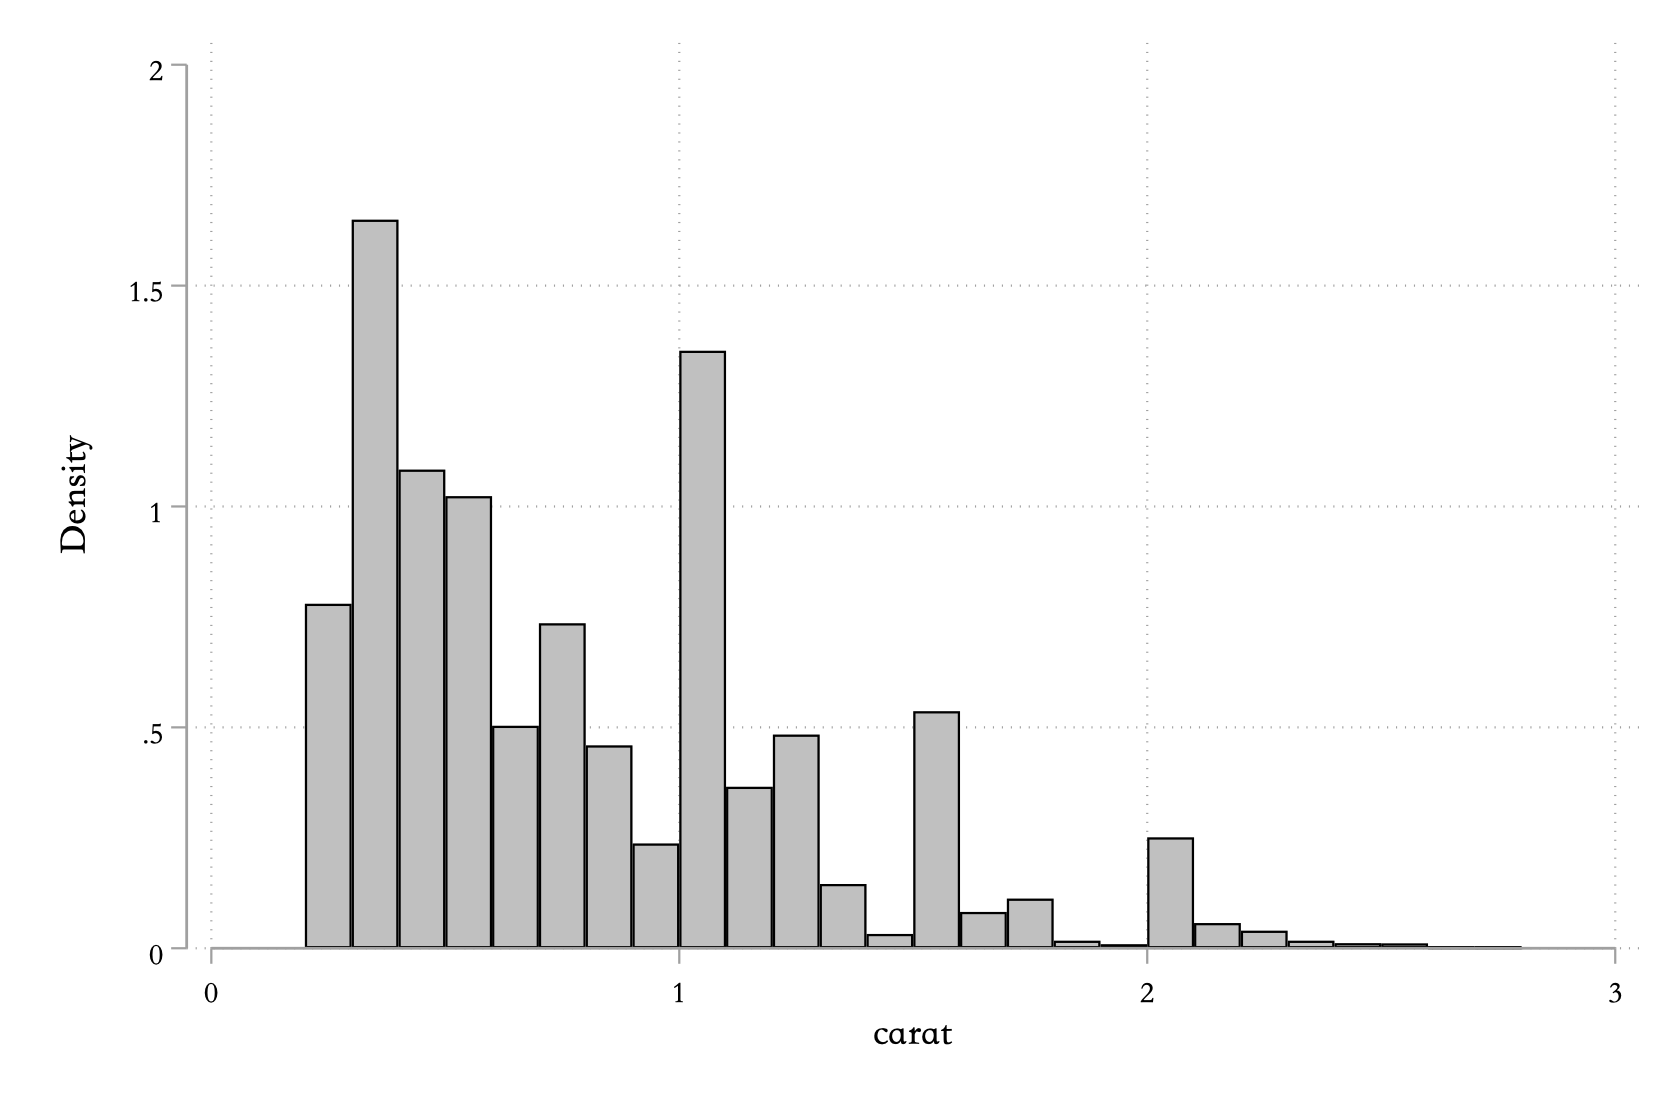
\includegraphics[width=\textwidth]{assets/histsmallercarat.png}
  \caption{carat < 3 子集中 carat 变量的分布}
  \label{fig:histsmallercarat}
\end{figure}

在同一幅图中叠加多个直方图是不好的,建议使用 kdensity 命令:

\begin{lstlisting}
use diamonds, clear
keep carat cut
colorscheme 5, palette(Paired)
tw ///
kdensity carat if cut == 1, lc("`r(color1)'") lp(solid) || ///
kdensity carat if cut == 2, lc("`r(color2)'") lp(solid) || ///
kdensity carat if cut == 3, lc("`r(color3)'") lp(solid) || ///
kdensity carat if cut == 4, lc("`r(color4)'") lp(solid) || ///
kdensity carat if cut == 5, lc("`r(color5)'") lp(solid) ||, ///
leg(order(1 "Fair" 2 "Good" 3 "Very Good" 4 "Premium" 5 "Ideal")) ///
xti("carat") yti("density") ylab(, format(%6.2f))
\end{lstlisting}

\begin{figure}[htbp]
  \centering
  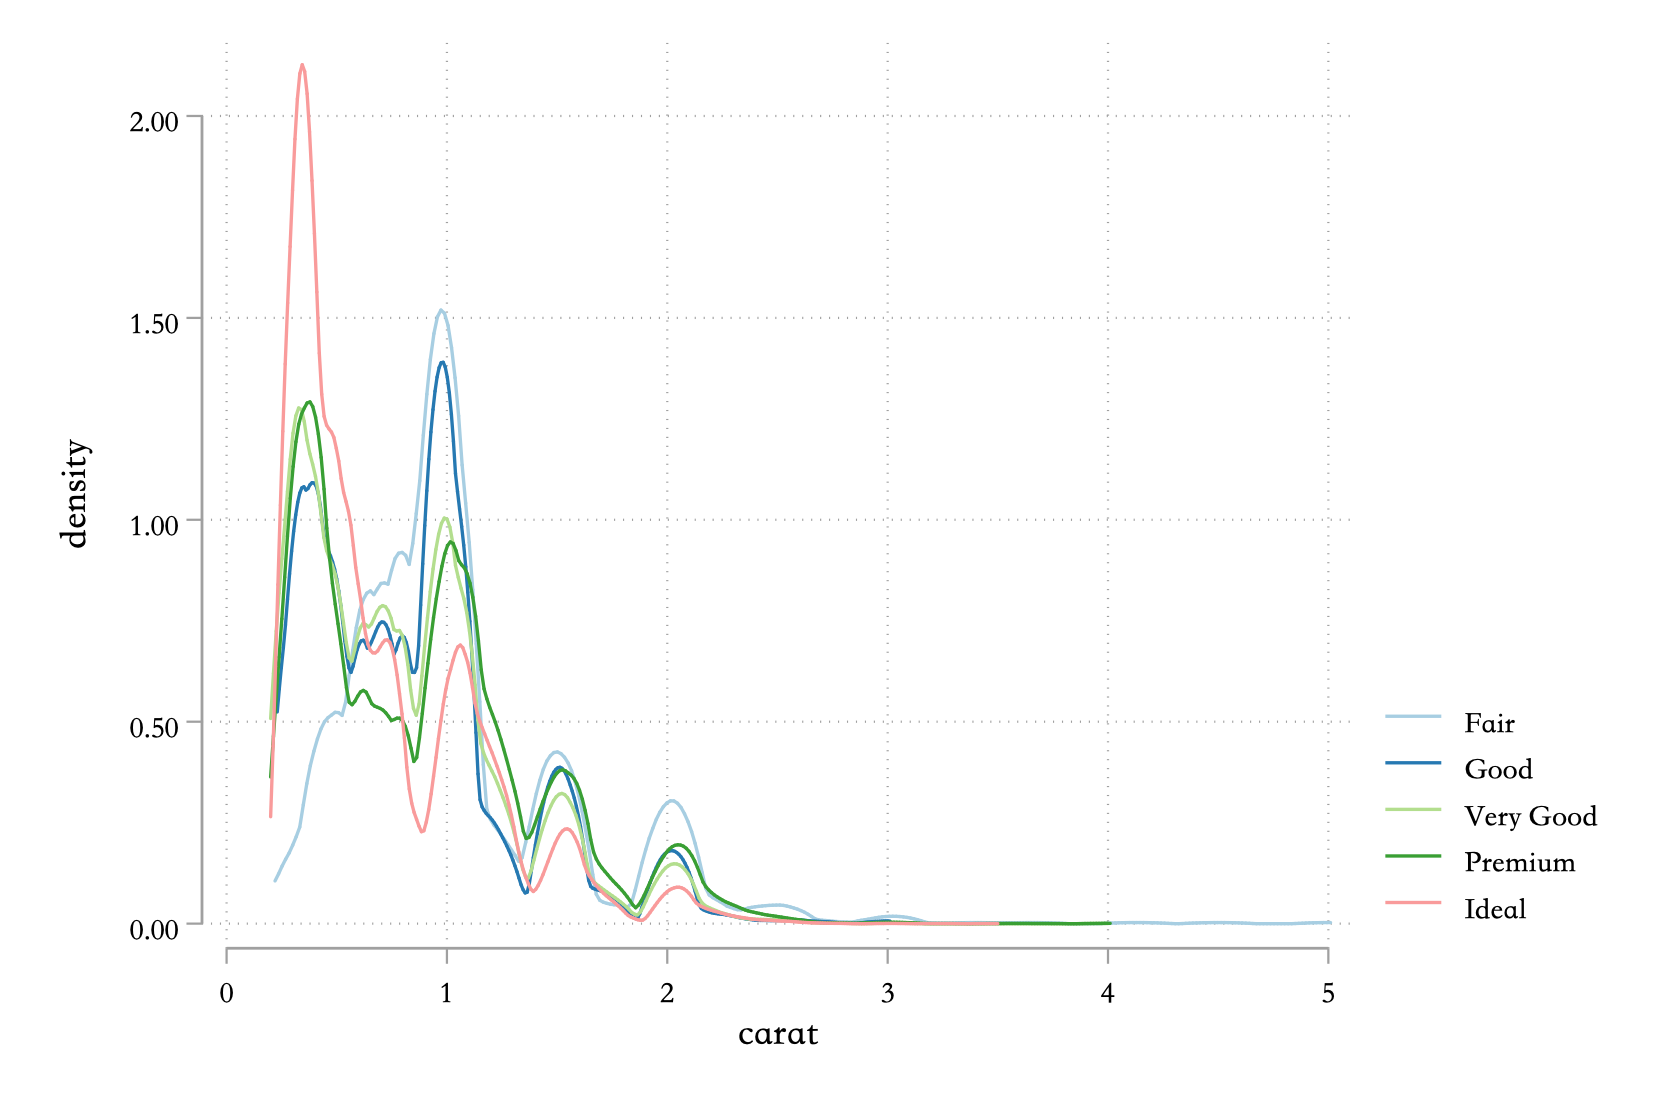
\includegraphics[width=\textwidth]{assets/kdensitycarat.png}
  \caption{carat 变量的核密度分布}
  \label{fig:kdensitycarat}
\end{figure}
